\documentclass[11pt,a4paper]{report}

% Aberstwyth dissertation LaTeX Template
% Authors: Dr. Hannah Dee (hmd1@aber.ac.uk), Neil Taylor (nst@aber.ac.uk)
% This has been adapted from the Leeds Thesis template and the 
% Group Project template for Computer Science in Aberystywth University.
% 
% All comments and suggestions welcome.
%
% Template designed to be used with pdflatex: it may need alteration to
% run with a different LaTeX engine

% To build document on the unix command line, run four commands:
 
% pdflatex dissertation
% bibtex dissertation
% pdflatex dissertation
% pdflatex dissertation

% you will end up with dissertation.pdf 
\usepackage{mmp}
\usepackage{fontspec} % Provide features for AAT and OpenType fonts
 \setmainfont{Helvetica Neue Light}
 
% the following packages are used for citations - You only need to include one. 
%
% Use the cite package if you are using the numeric style (e.g. IEEEannot). 
% Use the natbib package if you are using the author-date style (e.g. authordate2annot). 
% Only use one of these and comment out the other one. 
\usepackage{cite}
%\usepackage{natbib}

% Use the following to selectively exclude chapters
%\includeonly{cover,abstract,acknowledge,declare,chapter1,chapter2}

\begin{document}

% all of the include directives below refer to tex files
% so 
\title{Tonight - An iOS app for event aggregation}

% Your name
\author{Ryan Clarke}

% Your email 
\authoremail{ryc@aber.ac.uk}

\degreeschemecode{G401} %e.g. G400 
\degreeschemetitle{Computer Science} % e.g. Computer Science
\degreetype{BSc}

\modulecode{CS39440} % i.e. CS39440, CC39440, CS39620
\moduletitle{Major Project} % i.e. Major Project or Minor Project

\date{8th April 2014} % i.e. the date of this version of the report

\status{Draft} % Use draft until you create the release version. Then, change this to Release.
\version{1.0}

%The title and name of your supervisor.
\supervisor{Dr. Richard Jensen} 

%The email for your supervisor. 
\supervisoremail{rkj@aber.ac.uk}

\maketitle



 includes cover.tex - to change the content,
% edit the tex file

\pagenumbering{roman}

% This is the front page

\title{Tonight - An iOS app for event aggregation}

% Your name
\author{Ryan Clarke}

% Your email 
\authoremail{ryc@aber.ac.uk}

\degreeschemecode{G401} %e.g. G400 
\degreeschemetitle{Computer Science} % e.g. Computer Science
\degreetype{BSc}

\modulecode{CS39440} % i.e. CS39440, CC39440, CS39620
\moduletitle{Major Project} % i.e. Major Project or Minor Project

\date{8th April 2014} % i.e. the date of this version of the report

\status{Draft} % Use draft until you create the release version. Then, change this to Release.
\version{1.0}

%The title and name of your supervisor.
\supervisor{Dr. Richard Jensen} 

%The email for your supervisor. 
\supervisoremail{rkj@aber.ac.uk}

\maketitle



                        

% Set up page numbering
\pagestyle{empty}

% declarations of originality 
\thispagestyle{empty}

%%%
%%% You must sign the declaration of originality. 
%%%
\begin{center}
    {\LARGE\bf Declaration of originality}
\end{center}

In signing below, I confirm that:

\begin{itemize}
\item{This submission is my own work, except where clearly
indicated.  }

\item{I understand that there are severe penalties for plagiarism 
and other unfair practice, which can lead to loss of marks
or even the withholding of a degree. }
 
\item{I have read the sections on unfair practice in the Students' 
Examinations Handbook and the relevant sections of the 
current Student Handbook of the Department of Computer 
Science.}
 
\item{I understand and agree to abide by the University's
regulations governing these issues.}
\end{itemize}

\vspace{3em}
Signature ............................................................  \\

\vspace{1em}
Date ............................................................ \\

%%% 
%%% We would like to make a selection of final reports available to students that take 
%%% this module in future years. To enable us to do this, we require your consent. You 
%%% are not required that you do this, but if you do give your consent, then we will have 
%%% the option to select yours as one of a number of reports as examples for other 
%%% students. If you would like to give your consent, then please include the following 
%%% text and sign below. If you do not wish to give your consent, please remove this 
%%% from your report. 
%%%
\vspace{5em}
\begin{center}
    {\LARGE\bf Consent to share this work}
\end{center}

In signing below, I hereby agree to this dissertation being made available to other
students and academic staff of the Aberystwyth Computer Science Department.  

\vspace{3em}
Signature ............................................................  \\

\vspace{1em}
Date ............................................................ \\

               

\thispagestyle{empty}

\begin{center}
    {\LARGE\bf Acknowledgements}
\end{center}

I would like to thank my dissertation tutor Richard Jensen for helping throughout the project.

I would also like to thank my parents for the support they have given me throughout my degree.
 % Acknowledgements
\thispagestyle{empty}

\begin{center}
    {\LARGE\bf Abstract}
\end{center}

This report describes a project for helping users find events around them. When visiting  a new area trying to find out what's going on can be difficult even for the most adept regular. Tonight tries to solve that problem by providing a mobile application that allows you to discover events that are going on around you. It does this by presenting the user with events that may be of interest to them via a `My Feed' section. A user also has the ability to explore events by selecting a city/area then drilling down to a particular venue or category. The users is then able to view all of the details on a particular event, with the option to follow the event. By following an event the system can learn about the user and present them with suggestions of events, based on what similar users are also following. To do this I developed a Ruby on Rails server application that provided a REST based API to access the information that a user needed, as part of this I also developed a data mining module to be able to pull in information from various data sources. Using this in conjunction with an iOS application to present the data and add in functionality to the user on a mobile device.                  % Abstract

\pagenumbering{roman}
\pagestyle{fancy}
\fancyhead{}
\fancyfoot[C]{\thepage}
\renewcommand{\headrulewidth}{0 pt}
\renewcommand{\chaptermark}[1]{\markboth{#1}{}}

\tableofcontents   
\newpage
\listoffigures
\newpage 
\listoftables
\newpage

% Set up page numbering
\pagenumbering{arabic}

\setchapterheaderfooter

% include the chapters
\chapter{Background \& Objectives}

This section should discuss your preparation for the project, including background reading, your analysis of the problem and the process or method you have followed to help structure your work.  It is likely that you will reuse part of your outline project specification, but at this point in the project you should have more to talk about. 

\textbf{Note}: 

\begin{itemize}
   \item All of the sections and text in this example are for illustration purposes. The main Chapters are a good starting point, but the content and actual sections that you include are likely to be different.
   
   \item Look at the document on the Structure of the Final Report for additional guidance. 
   
\end {itemize}

\section{Background}
What was your background preparation for the project? What similar systems did you assess? What was your motivation and interest in this project? 

\section{Analysis}
Taking into account the problem and what you learned from the background work, what was your analysis of the problem? How did your analysis help to decompose the problem into the main tasks that you would undertake? Were there alternative approaches? Why did you choose one approach compared to the alternatives? 

There should be a clear statement of the objectives of the work, which you will evaluate at the end of the work. 

In most cases, the agreed objectives or requirements will be the result of a compromise between what would ideally have been produced and what was felt to be possible in the time available. A discussion of the process of arriving at the final list is usually appropriate.

\section{Process}
You need to describe briefly the life cycle model or research method that you used. You do not need to write about all of the different process models that you are aware of. Focus on the process model that you have used. It is possible that you needed to adapt an existing process model to suit your project; clearly identify what you used and how you adapted it for your needs.


%\addcontentsline{toc}{chapter}{Development Process}
\chapter{Design}
	There are 2 main parts of the project the first being the server element and the second the mobile application itself. The mobile application will be connecting to the server applications through a RESTFull API to retrieve all of the data that's required. The server element will be composed of 3 main parts the RESTFull API, Administration panel, and the data mining part.
	\begin{figure}[ht] % H - For exact position 
			\caption[Overview design]{This diagram shows the main areas of the project and how the interact with each other. }
			\centering
			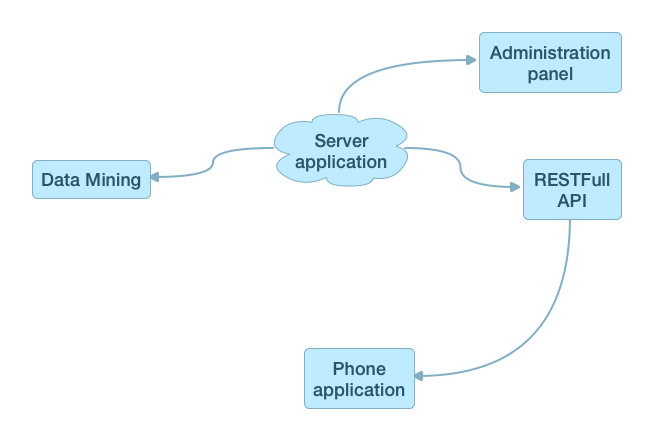
\includegraphics[width=0.5\textwidth]{Images/overview-design}
			\label{fig:overview-design}
		\end{figure}
	
	\section{Database}
		To full fill the requirement of utilising a cloud server solution the database will be using PostgresSQL which the server element will interface with it using the ActiveRecord gem bundled with Ruby on Rails. Because the server element was designed using TDD and each the overall design, was moulded during the process Figure \ref{fig:erd} shows the resultant entity relationship diagram at the end of the project. There is also a set of definite fields that was worked from the Facebook API schema listed in Table \ref{fig:facebookEventVenues}, schema.org\cite{schemaEvent} was also used to help build the list of relevant information on an event. 

		\begin{figure}[ht] % H - For exact position 
			\caption[Entity Relationship Diagram]{This diagram depicts the various entities, and their interactions with each other.}
			\centering
			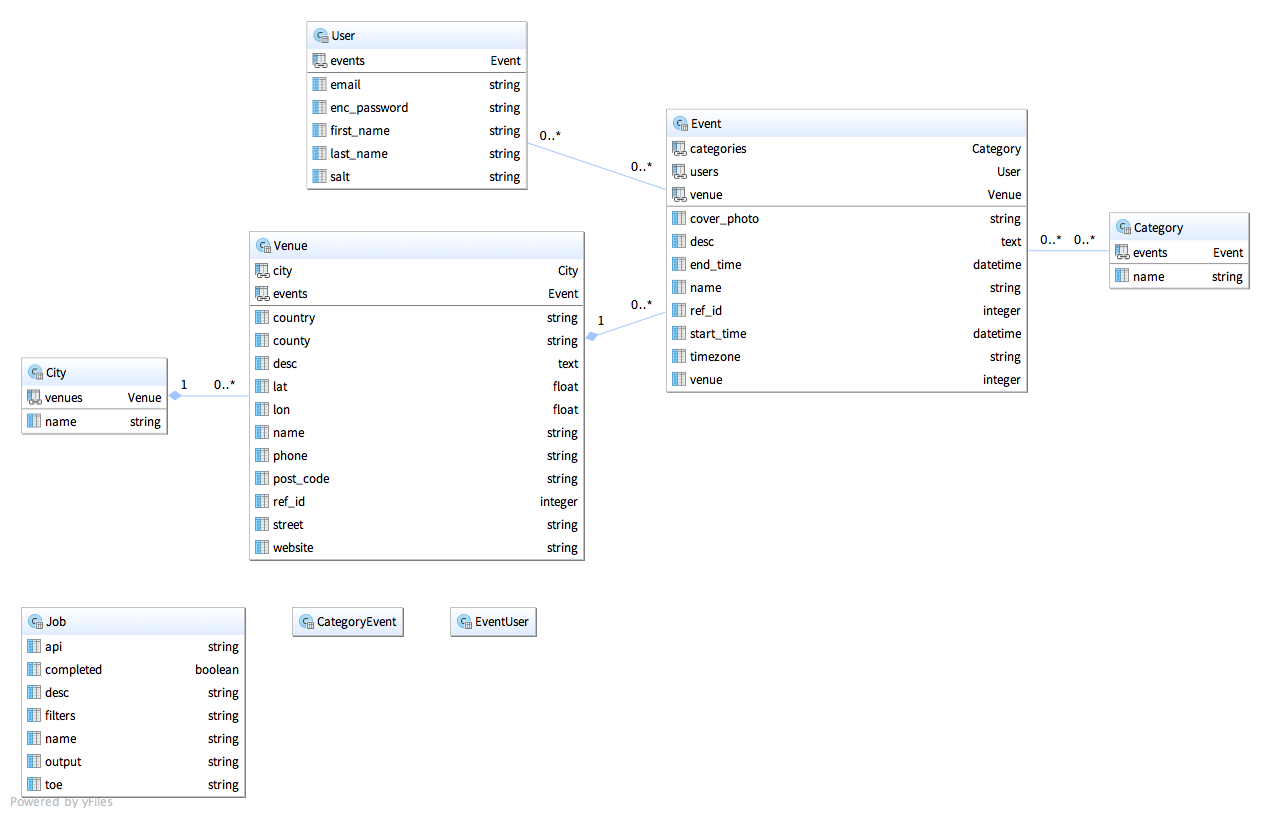
\includegraphics[width=1\textwidth,angle=90]{Images/ERD}
			\label{fig:erd}
		\end{figure}

	\section{Server Application}
		The server application, will be composed of 3 components these will be the Data mining module, the RESTFull API for interfacing with the mobile application, and the administration panel. These components whilst being separate, will all interact with the same database and will reside within the same code base to be uploaded and ran on the cloud application platform (CAP).

		\subsection{Development tools}
			The server application will be written in Ruby utilising the Ruby on Rails (RoR) framework, there were other options to use such as; Node, Clojure, Java, Python. However the RoR framework provided great native support for developing API's and database integration. Rails also gives us the ability to run code using the rails environment via the command line by use of rake tasks. The CAP will call the task hourly using a cron job to pull in new events and venues, these jobs will be specified by the administration panel and then ran by the rake task. 

			To develop the server side code the programmer will be using the Sublime Text 2 text editor\cite{sublime} with the following packages installed; RSpec\cite{RSpecSub}, Ruby Test\cite{RubyTest}, and Rails Developer Snippets\cite{RDS}. These packages will assist the programmer by allowing them to run tests within the editor and provide key snippets to be used by them. The use of a text editor with the packages noted installed allowed a cleaner interface for the programmer to deal with and was a tool they where familiar with. 

			As stated above, the programmer will be following a test driven development approach as such it will be required to use some form of test framework. For this the programmer will be using RSpec for RoR gem\cite{RSpecRails}, this gem provides the user with the RSpec suite correctly optimised and set-up to be used within a RoR environment. The programmer will also be using FactoryGirl\cite{FactoryGirl} a higher grain of control over mock models, and WebMock\cite{WebMock} to be able to mock API connections with test data. 

		\subsection{OAuth}
			The application will use the OAuth standard for authentication to the application, OAuth is an open protocol that offers `secure client delegation'. By delegating a different user token for each user the server can serve user specific data to each user, whilst ensuring statelessness. The use of OAuth will also restrict server resources to defined applications, allowing a higher level of control to the applications that utilise the API. 

		\subsection{Routes}
			Ruby on Rails allows for a series of URL routes to be defined, to ensure the project follows REST principles the API the interface is required to be uniform, for this all requests will be responded in JSON and will be in the format similar to snippet \ref{fig:JSONOutput}. The API URI structure should also be representational of the data being served and how the data is structured in the database. Table \ref{fig:apiRoutesTable} shows the endpoints and accessors for the data that's available through the API. The returned data will also be paginated using the gem api-pagination\cite{paginate} the pagination URIs will be formed as part of the header information of the response to keep the returned body easy to parse. 

			\begin{program}
				\begin{verbatim}
				{
					`code' => `201',
					`errors' => `',
					`body' => [ ]
				}
				\end{verbatim}
				\caption{Example JSON output for REST requests}
				\label{fig:JSONOutput}
			\end{program}

			\begin{table}[h]
				\centering
				\caption{API Routes}
				\begin{tabular}{|l|l|l|}
				\hline
				Verb &  URI Pattern                                      &  Controller\#Action                           \\ \hline
				GET  &    /api/v1/events(.:format)                       &                     api/v1/events\#index      \\
				GET  &    /api/v1/events/:id(.:format)                   &                 api/v1/events\#eventByID      \\
				GET  &     /api/v1/venues(.:format)                      &                      api/v1/venues\#index     \\
				GET  &     /api/v1/venues/:id(.:format)                  &                  api/v1/venues\#show          \\
				GET  &     /api/v1/venues/:id/events(.:format)           &           api/v1/events\#eventsByVenue        \\
				POST &    /api/v1/register(.:format)                     &                    api/v1/user\#register      \\
				GET  &     /api/v1/user(.:format)                        &                        api/v1/user\#index     \\
				POST &    /api/v1/user(.:format)                         &                       api/v1/user\#update     \\
				GET  &     /api/v1/user/feed(.:format)                   &                  api/v1/user\#feed            \\
				GET  &     /api/v1/user/following(.:format)              &              api/v1/following\#index          \\
				POST &    /api/v1/user/follow(.:format)                  &                 api/v1/following\#followEvent \\
				POST &    /api/v1/user/unfollow(.:format)                &               api/v1/following\#unfollowEvent \\ 
				GET  &    /api/v1/categories(.:format)                   &                  api/v1/categories\#index     \\
				GET  &     /api/v1/categories/:id(.:format)              &              api/v1/categories\#show          \\
				GET  &     /api/v1/categories/:id/events(.:format)       &      api/v1/events\#eventsByCategory          \\
				GET  &     /api/v1/cities(.:format)                      &                      api/v1/cities\#index     \\
				GET  &     /api/v1/cities/:id(.:format)                  &                  api/v1/cities\#show          \\
				GET  &     /api/v1/cities/:id/events(.:format)           &           api/v1/events\#eventsByCity         \\
				GET  &     /api/v1/cities/:city\_id/venues(.:format)     &     api/v1/venues\#venuesByCity               \\
				GET  &     /api/v1/cities/:city\_id/categories(.:format) &  api/v1/categories\#catsByCity                \\ \hline
				\end{tabular}
				\label{fig:apiRoutesTable}
			\end{table}

			% \begin{table}
			% 	\centering
			% 	\caption{OAuth Routes}
			% 	\begin{tabular}{|l|l|l|}
			% 	\hline
			% 	GET    &     /oauth/authorize/:code(.:format)           &             doorkeeper/authorizations\#show           \\ \hline
			% 	GET    &     /oauth/authorize(.:format)                 &                    doorkeeper/authorizations\#new     \\
			% 	POST   &    /oauth/authorize(.:format)                  &                    doorkeeper/authorizations\#create  \\
			% 	PATCH  &   /oauth/authorize(.:format)                   &                    doorkeeper/authorizations\#update  \\
			% 	PUT    &     /oauth/authorize(.:format)                 &                    doorkeeper/authorizations\#update  \\
			% 	DELETE &  /oauth/authorize(.:format)                    &                    doorkeeper/authorizations\#destroy \\
			% 	POST   &    /oauth/token(.:format)                      &                        doorkeeper/tokens\#create      \\
			% 	GET    &     /oauth/applications(.:format)              &                 doorkeeper/applications\#index        \\
			% 	POST   &    /oauth/applications(.:format)               &                 doorkeeper/applications\#create       \\
			% 	GET    &     /oauth/applications/new(.:format)          &             doorkeeper/applications\#new              \\
			% 	GET    &     /oauth/applications/:id/edit(.:format)     &        doorkeeper/applications\#edit                  \\
			% 	GET    &     /oauth/applications/:id(.:format)          &             doorkeeper/applications\#show             \\
			% 	PATCH  &   /oauth/applications/:id(.:format)            &             doorkeeper/applications\#update           \\
			% 	PUT    &     /oauth/applications/:id(.:format)          &            doorkeeper/applications\#update            \\
			% 	DELETE &  /oauth/applications/:id(.:format)             &             doorkeeper/applications\#destroy          \\
			% 	GET    &     /oauth/authorized\_applications/  &      doorkeeper/authorized\_applications\#index       \\
			% 	DELETE &  /oauth/authorized\_applications/:id &  doorkeeper/authorized\_applications\#destroy         \\
			% 	GET    &     /oauth/token/info(.:format)                &                   doorkeeper/token\_info\#show        \\ \hline
			% 	\end{tabular}
			% 	\label{fig:OAuthRoutesTable}
			% \end{table}
		
		\subsection{Data mining element}
			The data mining element is broken up into a 2 different parts these being the interfaces to the external data sources, and the second being the job scheduler. Figure \ref{fig:mining} shows how these parts will work together to input data from the various API's that's needed. To allow for any number of API's to be added to the system, a base class called `Resources' will be needed with any inherited functions needed Figure \ref{fig:class_api} shows the class diagram for this part of the project. Then another class that inherited from `Resources' will be used to define each individual API connection. By doing this the API is easy to extend simply by working as a interpreter to the different names for data fields and layout for each API response. The scheduler RAKE  task will then read in the jobs defined by the administration panel and pull in the relevant information and insert this into the database.

			\begin{figure}[ht] % H - For exact position 
				\caption[Class Diagram for API integration ]{This diagram describes the functions and inheritance used for the library that connects to the APIs}
				\centering
				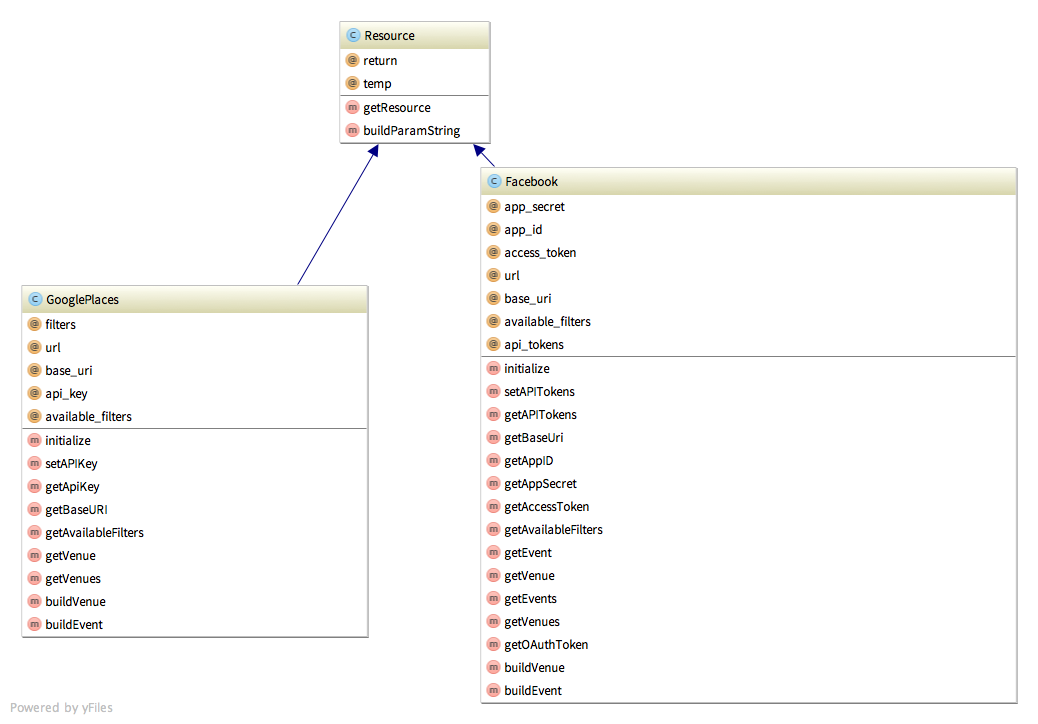
\includegraphics[width=1\textwidth]{Images/resources}
				\label{fig:class_api}
			\end{figure}

			\begin{figure}[ht] % H - For exact position 
				\caption[Overview of the data mining aspect]{This diagram shows an overview of how the different data mining module is composed.}
				\centering
				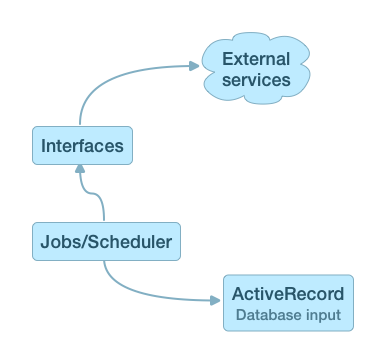
\includegraphics[width=0.5\textwidth]{Images/mining-overview}
				\label{fig:mining}
			\end{figure}

		\subsection{Class diagram}
			Following on from the MVC design pattern and the fact the API needs to be representational, each controller is representational for each table stored in the database. However in some cases there are filters such as being able to get the events via the venue, since this will return a list of events rather than venues the method to do this is inside the events controller. Figure \ref{fig:controllers} shows the structure of the controllers, and the methods inside of them. 

			\begin{figure}[ht] % H - For exact position 
				\caption[Controllers Class Diagram]{This diagram shows the classes along with the methods and class variables}
				\centering
				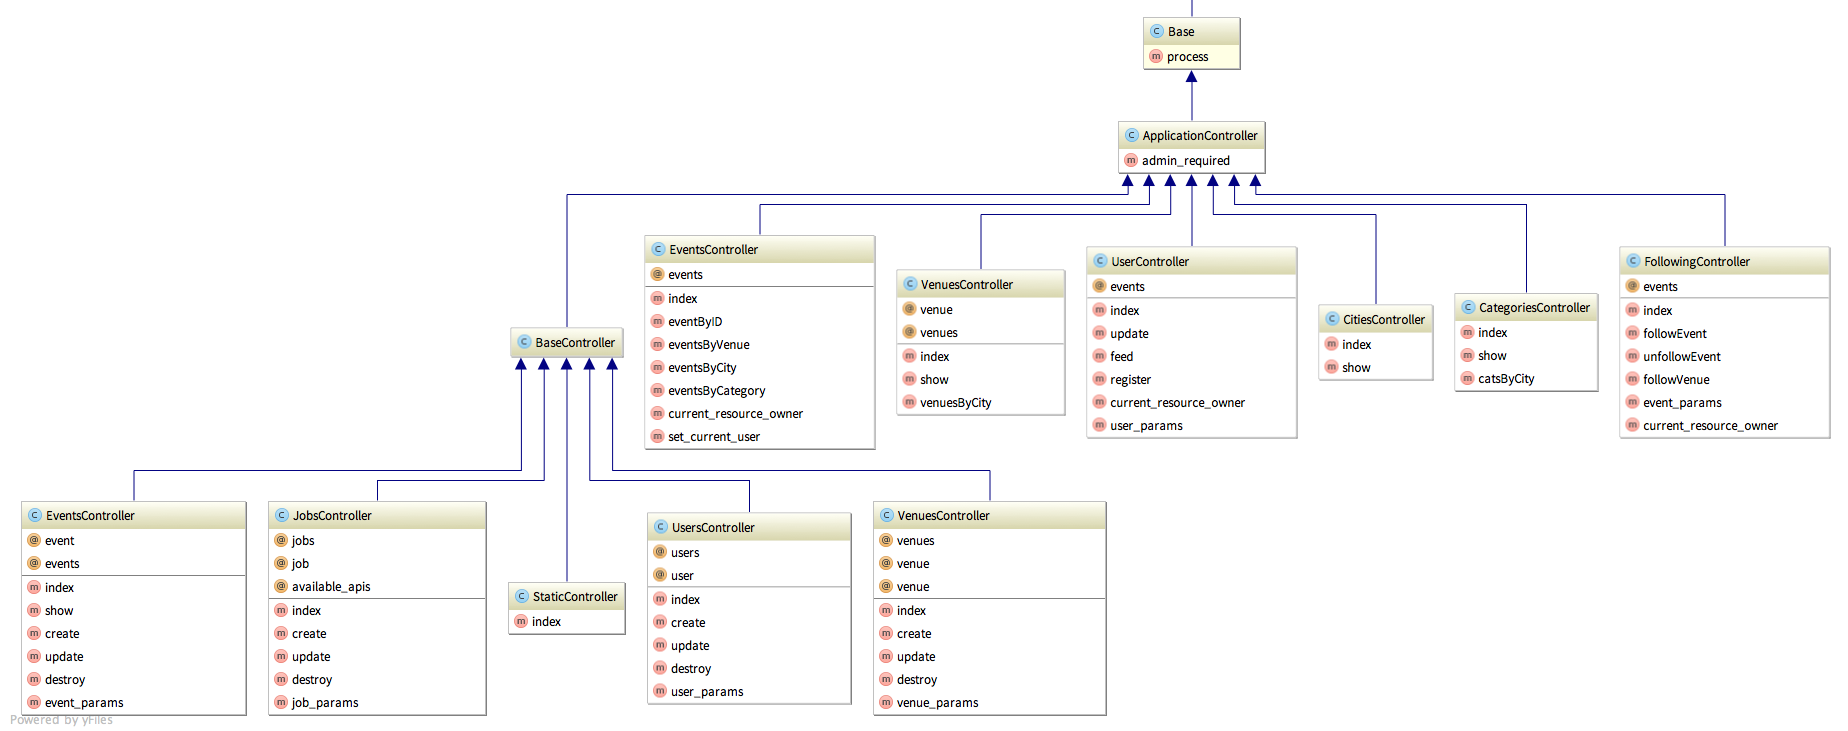
\includegraphics[width=1\textwidth,angle=90]{Images/controllers_crop}
				\label{fig:controllers}
			\end{figure}


	\section{iOS Application}

		\subsection{Development tools}
			To develop in iOS you are required to use Apples own IDE XCode, version 5 is the latest and supports the latest version of iOS. XCode 5 includes a number of tools bundled with the IDE including the iOS Simulator and GIT Integration. Cocoa pods will also be used for package management and pulling in various libraries that will be used throughout the project. XCode 5 itself is a purpose built IDE for iOS applications and everything that was required came as standard and was used as a one stop solution for the development of the mobile application. 

		\subsection{Wireframes}
			The main application will consist of 2 main views these being a list of events with some filter applied and the event details themselves. Figure \ref{fig:wireframes} depicts a rough outline of where elements will be positioned and the possible interactions a user can undertake. Figure \ref{fig:multi-events} shows the various different ways I could present the data using the iOS' table view to show list events happening, the list of events screen will be re-usable and able to show a list of events with a wide range of filters applied to it. The filters applied will be dependant on how the user access the list view be it through the `Discover' tab or the `My Feed' tab. 

			The wireframes show the 3 key different screens, the first being the `My Feed' tab  this tab is used to show the users personalised feed, this will utilise the list view for the events and then when an event is selected it will show the user the selected event using the individual event view. The second is the `Discover' tab this will be used to be able to select events from a particular city, it will then give you the option to select a particular category or venue to see relevant events to the selector chosen. The third is the `My Profile' tab this will be where you can see your information potentially change it and view the events you are following, this will also present you with the option to `unfollow' these events as well.

			\begin{figure}[H]
				\centering
				\caption{Basic wireframes and design choices for the mobile application}
				\begin{minipage}{.5\linewidth}
					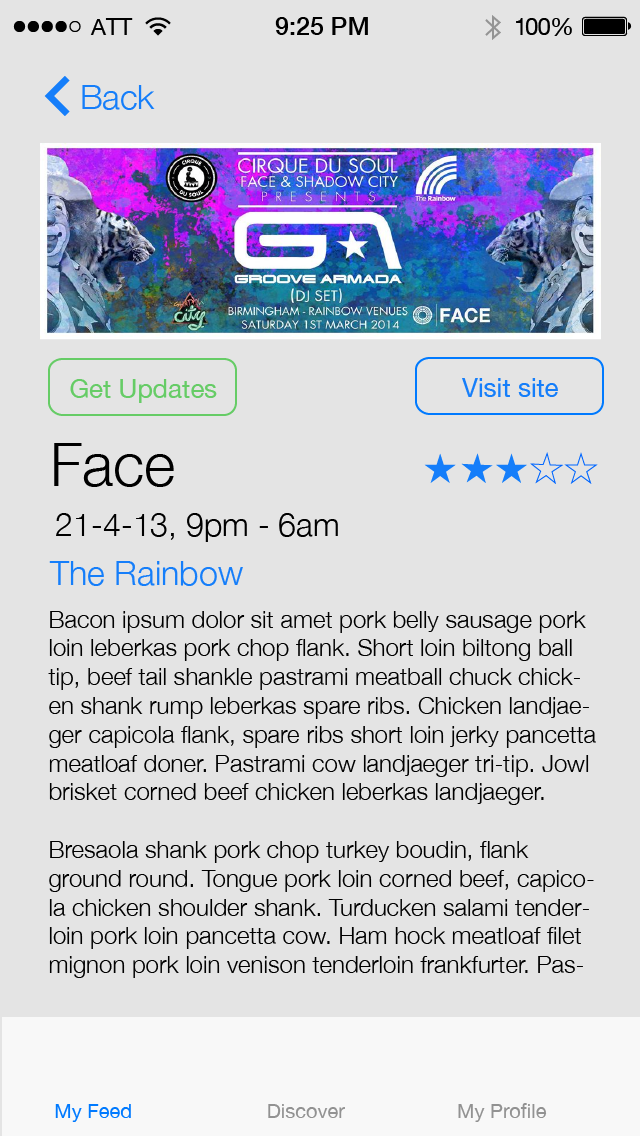
\includegraphics[width=0.9\textwidth]{Images/indiv-event}
					\caption{Individual event wireframe}
					\label{fig:indiv-event}
				\end{minipage}%
				\begin{minipage}{.5\linewidth}
					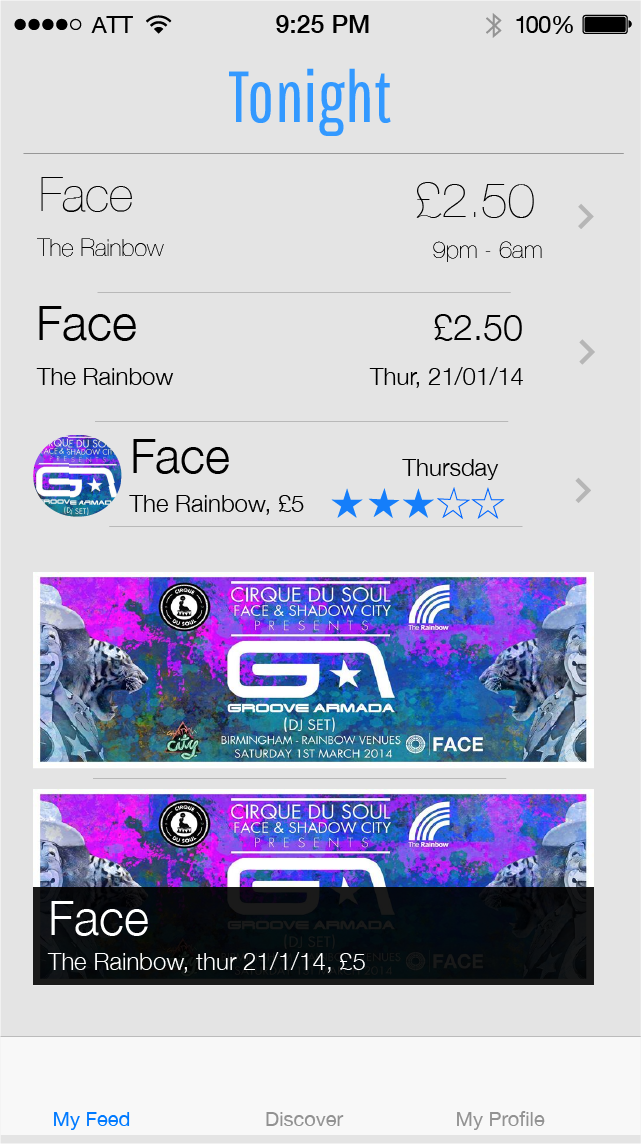
\includegraphics[width=0.9\textwidth]{Images/multi-events}
					\caption{List of events wireframe}
					\label{fig:multi-events}
				\end{minipage}
				\label{fig:wireframes}
			\end{figure}

		\subsection{Class diagrams}
			The majority of the application design was based on the delegation design pattern where actions and data are linked with the UI elements, and so the mobile application is a series of controllers where it retrieves information and outputs this into the UI. There will be a different controller for each screen that can be viewed as part of the application. Including this I will be using data classes to store and use the data pulled in from the server. Figure \ref{fig:ios-data} shows the 2 classes I will be using to keep the data retrieved from the API, these classes are simple data classes that have some functionality applied to them and allow for scope as the project develops. 

			\begin{figure}
				\centering
				\caption{Class diagram for the iOS data classes}
				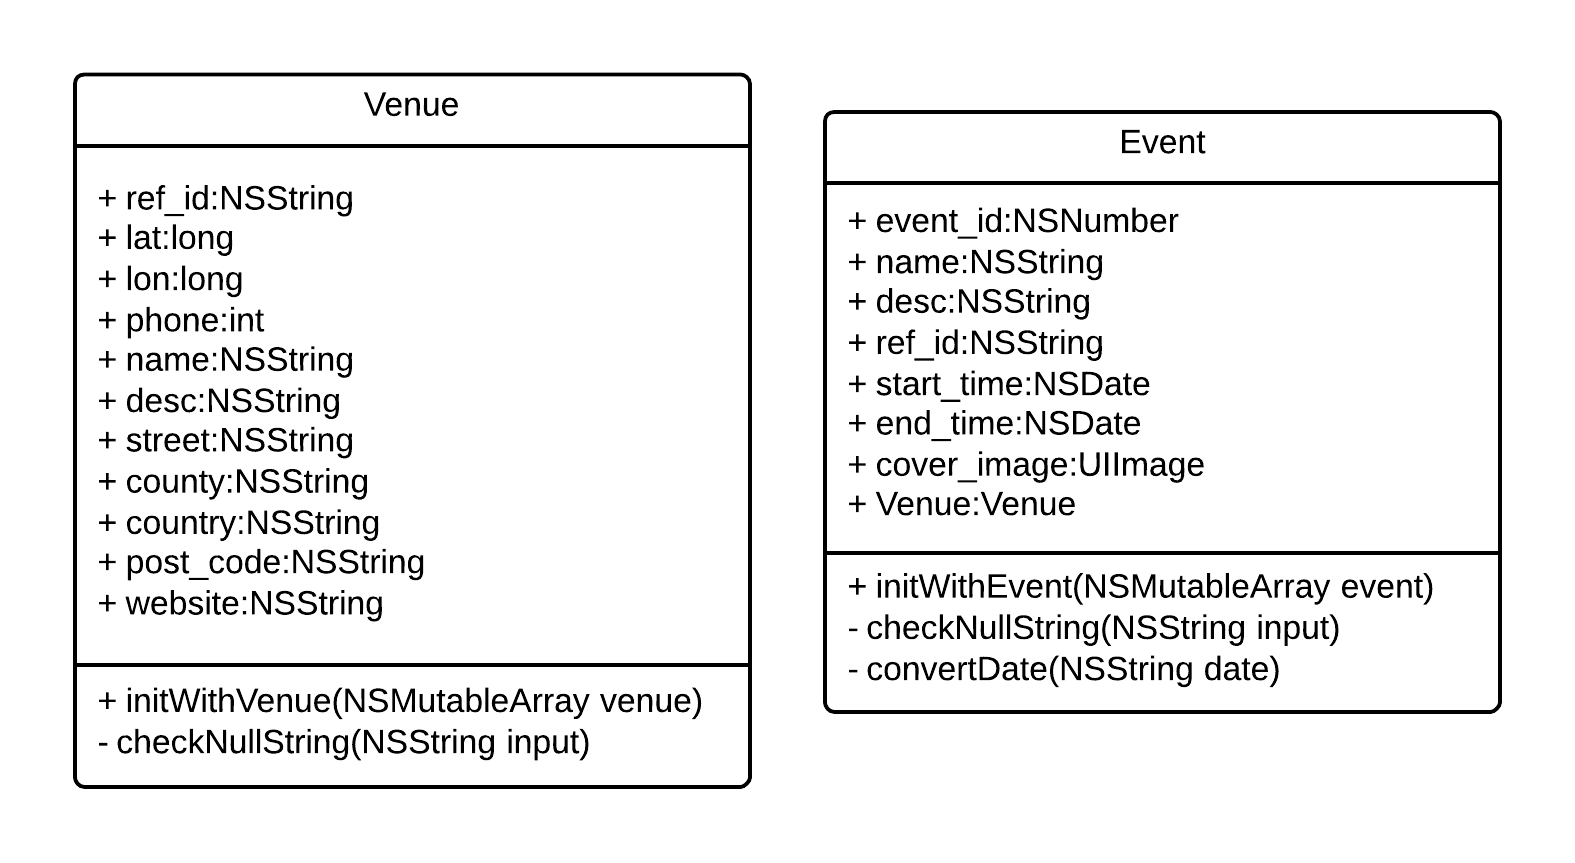
\includegraphics[width=0.6\linewidth]{Images/ios-data}
				\label{fig:ios-data}
			\end{figure}
\chapter{Implementation}

The implementation should look at any issues you encountered as you tried to implement your design. During the work, you might have found that elements of your design were unnecessary or overly complex; perhaps third party libraries were available that simplified some of the functions that you intended to implement. If things were easier in some areas, then how did you adapt your project to take account of your findings?

It is more likely that things were more complex than you first thought. In particular, were there any problems or difficulties that you found during implementation that you had to address? Did such problems simply delay you or were they more significant? 

You can conclude this section by reviewing the end of the implementation stage against the planned requirements. 
\chapter{Testing}

	This section describes the approach to testing undertaken throughout the project, along with some results from the tests that where undertaken.

\section{Overall Approach to Testing}
	To develop the server side element of the project the programmer followed a test driven approach utilising the red-green-refactor principle.  By doing this it enabled the code to be as efficient as possible whilst still undertaking the task that block of code was expected to do. This method was chosen as the majority of the code required on the server side application didn't utilise a GUI and benefited from a much more pragmatic  approach to testing. As part of the server element had to pull in information from external sources `WebMock' was used to mock HTTP connections to the external API's, this was used to serve test data to the code and to be able to check any transformations on the data. 

	To develop the mobile application a more behaviour driven approach was used, by writing the code and conducting  a manual test seemed the more logical way. As most of the code was by use of target-action concept, meaning that the bulk of code was methods to be ran when a particular button is selected in the GUI. This also helped with the requirement testing, by ensuring that the requirements where in place and functioning on the mobile device itself. 
	
\section{Automated Testing}
	To conduct the automated tests on the server element of the project I used RSpec which is a testing environment for Ruby. RSpec has a version that's designed for the use within Ruby on Rails of which is the version used, RSpec gives the programmer the ability to test all aspects of the code including models, controllers and views. The programmer first wrote the tests that where needed for a particular feature or element of the program, and then implemented the function. However sometimes the test needed to be reviewed to ensure that it was testing the code correctly as, occasional odd results would appear after implementing a feature. 
	
\subsection{Other types of testing}

\subsection{Stress Testing}
	Stress testing the server side element is pretty irrelevant due to the nature of the cloud based server it's running on we almost have unlimited resources to utilise if the server comes under significant stress. Heroku gives you the ability to add and remove physical resources such as CPU power and RAM whenever the demand is so high it's required. With the current scale of the application there is plenty of leeway to supply to the potential demand. If this demand became more persistent then it would be an adequate time to ensure the code is running as leanly as possible. 

	XCode 5 gives some great tools to be able to visualise how well the application is running on the mobile device, 

	% Run app in XCode and test from there.

\section{Integration Testing}
	For the most part the 



Detailed descriptions of every test case are definitely not what is required here. What is important is to show that you adopted a sensible strategy that was, in principle, capable of testing the system adequately even if you did not have the time to test the system fully.

Have you tested your system on real users? For example, if your system is supposed to solve a problem for a business, then it would be appropriate to present your approach to involve the users in the testing process and to record the results that you obtained. Depending on the level of detail, it is likely that you would put any detailed results in an appendix.

The following sections indicate some areas you might include. Other sections may be more appropriate to your project. 
\chapter{Evaluation}

Examiners expect to find in your dissertation a section addressing such questions as:

\begin{itemize}
   \item Were the requirements correctly identified? 
   \item Were the design decisions correct?
   \item Could a more suitable set of tools have been chosen?
   \item How well did the software meet the needs of those who were expecting to use it?
   \item How well were any other project aims achieved?
   \item If you were starting again, what would you do differently?
\end{itemize}

Such material is regarded as an important part of the dissertation; it should demonstrate that you are capable not only of carrying out a piece of work but also of thinking critically about how you did it and how you might have done it better. This is seen as an important part of an honours degree. 

There will be good things and room for improvement with any project. As you write this section, identify and discuss the parts of the work that went well and also consider ways in which the work could be improved. 

Review the discussion on the Evaluation section from the lectures. A recording is available on Blackboard. 
% add any additional chapters here

\setemptyheader
\addcontentsline{toc}{chapter}{Appendices}
\chapter*{Appendices}
\pagebreak

% start the appendix - sets up different numbering
\fancypagestyle{plain}{%
%\fancyhf{} % clear all header and footer fields
\fancyhead[L]{\textsl{Appendix\ \thechapter}}
\fancyhead[R]{\textsl{\leftmark}}}

\appendix
\fancyhead[L]{\textsl{Appendix\ \thechapter}}
\fancyhead[R]{\textsl{\leftmark}}
\fancyhead[C]{}
\fancyfoot[C]{\thepage}
\renewcommand{\headrulewidth}{0.4pt}
\renewcommand{\chaptermark}[1]{\markboth{#1}{}}

\fancyhead[L]{\textsl{Appendix\ \thechapter}}
\fancyhead[R]{\textsl{\leftmark}}
\fancyfoot[C]{{\thepage} of \pageref{LastPage}}

% include any appendices here
\chapter{Third-Party Code and Libraries}

\section{Server side libraries}

Ruby on Rails is the base framework I used for my server application, RoR comes packaged with a host of other libraries all used as well. 
\cite{mit}. The library is released using the MIT License 
\cite{rails}. This library was used without modification. 

The packages Kaminari and api-pagination where used to add in pagination to the project
\cite{mit}. Both libraries is released using the MIT License 
\cite{kaminari}. This library was used without modification. 
\cite{paginate}. This library was used without modification. 

The packages RSpec, FactoryGirl, WebMock, spork-rails, guard-spork, and childprocess where all used as part of the testing setup. 
\cite{mit}. All libraries where released under the MIT LIcense.
\cite{rspec}. This library was used without modification. 
\cite{FactoryGirl}. This library was used without modification. 
\cite{WebMock}. This library was used without modification. 
\cite{spork}. This library was used without modification. 
\cite{child}. This library was used without modification. 

The httparty library was used to connect to external APIs
\cite{mit}. This library where released under the MIT LIcense.
\cite{httparty}. This library was used without modification. 

\section{Mobile application libraries}

UICKeyChainStore was used to store personal data using the iOS Key Chain
\cite{mit}. This library where released under the MIT LIcense.
\cite{keychain}. This library was used without modification. 

UniRest was used to retrieve data from the API over HTTP
\cite{mit}. This library where released under the MIT LIcense.
\cite{unirest}. This library was used without modification. 

MBProgressHUD was used to display a progress bar when undertaking certain tasks
\cite{mit}. This library where released under the MIT LIcense.
\cite{progress}. This library was used without modification. 

\chapter{Test Results}

\section{RSpec Results}

\begin{lstlisting}
...FF...F..*....*.......*..............*.........*.*.F.............*.......*..******..............*.*...........*

Pending:
  API::V1::UserController.feed Implement the feed
    # Not yet implemented
    # ./spec/controllers/api/v1/user_controller_spec.rb:45
  Admin::EventsController.update redirects to index after update
    # Not yet implemented
    # ./spec/controllers/admin/events_controller_spec.rb:46
  Admin::EventsController.create shows flash message when an error occurs
    # Not yet implemented
    # ./spec/controllers/admin/events_controller_spec.rb:31
  Admin::UsersHelper add some examples to (or delete) /Users/user/Dropbox/dissertation/code/server_software/tonight_server/spec/helpers/admin/users_helper_spec.rb
    # Not yet implemented
    # ./spec/helpers/admin/users_helper_spec.rb:14
  Admin::JobsController.create shows flash message when an error occurs
    # Not yet implemented
    # ./spec/controllers/admin/jobs_controller_spec.rb:35
  Admin::UsersController.update redirects to the index page
    # Not yet implemented
    # ./spec/controllers/admin/users_controller_spec.rb:50
  Admin::VenuesController.update redirects to the index page
    # Not yet implemented
    # ./spec/controllers/admin/venues_controller_spec.rb:46
  Admin::VenuesController.create shows flash message when an error occurs
    # Not yet implemented
    # ./spec/controllers/admin/venues_controller_spec.rb:31
  Venue add some examples to (or delete) /Users/user/Dropbox/dissertation/code/server_software/tonight_server/spec/models/venue_spec.rb
    # Not yet implemented
    # ./spec/models/venue_spec.rb:4
  FollowingControllerHelper add some examples to (or delete) /Users/user/Dropbox/dissertation/code/server_software/tonight_server/spec/helpers/following_controller_helper_spec.rb
    # Not yet implemented
    # ./spec/helpers/following_controller_helper_spec.rb:14
  Admin::EventsHelper add some examples to (or delete) /Users/user/Dropbox/dissertation/code/server_software/tonight_server/spec/helpers/admin/events_helper_spec.rb
    # Not yet implemented
    # ./spec/helpers/admin/events_helper_spec.rb:14
  Admin::VenuesHelper add some examples to (or delete) /Users/user/Dropbox/dissertation/code/server_software/tonight_server/spec/helpers/admin/venues_helper_spec.rb
    # Not yet implemented
    # ./spec/helpers/admin/venues_helper_spec.rb:14
  StaticHelper add some examples to (or delete) /Users/user/Dropbox/dissertation/code/server_software/tonight_server/spec/helpers/static_helper_spec.rb
    # Not yet implemented
    # ./spec/helpers/static_helper_spec.rb:14
  Admin::JobsHelper add some examples to (or delete) /Users/user/Dropbox/dissertation/code/server_software/tonight_server/spec/helpers/admin/jobs_helper_spec.rb
    # Not yet implemented
    # ./spec/helpers/admin/jobs_helper_spec.rb:14
  API::V1::FollowingController Implement the following venue stuff
    # Not yet implemented
    # ./spec/controllers/api/v1/following_controller_spec.rb:34
  API::V1::FollowingController.index responds with events logged in user follows
    # Not yet implemented
    # ./spec/controllers/api/v1/following_controller_spec.rb:20
  City add some examples to (or delete) /Users/user/Dropbox/dissertation/code/server_software/tonight_server/spec/models/city_spec.rb
    # Not yet implemented
    # ./spec/models/city_spec.rb:4

Failures:

  1) Facebook gets an event from it's ID
     Failure/Error: stub_request(:get, "https://graph.facebook.com/204504813084059/?access_token=accesstoken").to_return(:body => event);
     NameError:
       undefined local variable or method `event' for #<RSpec::ExampleGroups::Facebook_2:0x007f8e3f0532a8>
     # ./spec/facebook_spec.rb:49:in `block (2 levels) in <top (required)>'

  2) Facebook searches for various venues
     Failure/Error: expect(@facebook.getVenues(params)).to eq(venuesJSON);
       
       expected: {"data"=>[{"category"=>"Arts/entertainment/nightlife", "category_list"=>[{"id"=>"211155112228091", "name"=>"Event Venue"}, {"id"=>"191478144212980", "name"=>"Night Club"}, {"id"=>"179943432047564", "name"=>"Concert Venue"}], "name"=>"The Rainbow Venues", "id"=>"224699987546240"}], "paging"=>{"next"=>"https://graph.facebook.com/search?type=place&center=52.41649271,-4.07785633&distance=500&limit=5000&offset=5000&__after_id=134964199922380"}}
            got: [{"category"=>"Arts/entertainment/nightlife", "category_list"=>[{"id"=>"211155112228091", "name"=>"Event Venue"}, {"id"=>"191478144212980", "name"=>"Night Club"}, {"id"=>"179943432047564", "name"=>"Concert Venue"}], "name"=>"The Rainbow Venues", "id"=>"224699987546240"}]
       
       (compared using ==)
       
       Diff:
       @@ -1,3 +1,8 @@
       -"data" => [{"category"=>"Arts/entertainment/nightlife", "category_list"=>[{"id"=>"211155112228091", "name"=>"Event Venue"}, {"id"=>"191478144212980", "name"=>"Night Club"}, {"id"=>"179943432047564", "name"=>"Concert Venue"}], "name"=>"The Rainbow Venues", "id"=>"224699987546240"}],
       -"paging" => {"next"=>"https://graph.facebook.com/search?type=place&center=52.41649271,-4.07785633&distance=500&limit=5000&offset=5000&__after_id=134964199922380"},
       +[{"category"=>"Arts/entertainment/nightlife",
       +  "category_list"=>
       +   [{"id"=>"211155112228091", "name"=>"Event Venue"},
       +    {"id"=>"191478144212980", "name"=>"Night Club"},
       +    {"id"=>"179943432047564", "name"=>"Concert Venue"}],
       +  "name"=>"The Rainbow Venues",
       +  "id"=>"224699987546240"}]
       
     # ./spec/facebook_spec.rb:76:in `block (2 levels) in <top (required)>'

  3) Facebook gets a list of events from a venue
     Failure/Error: @facebook.getEvents("204504813084059").should eq(eventsJSON);
       
       expected: {"data"=>[{"name"=>"Godskitchen Presents Clash Of The Gods", "start_time"=>"2014-04-26T22:00:00+0100", "end_time"=>"2014-04-27T06:00:00+0100", "timezone"=>"Europe/London", "location"=>"The Rainbow Venues", "id"=>"204504813084059"}], "paging"=>{"cursors"=>{"after"=>"MzI5Mzc5MDYzODYwOTM5", "before"=>"MjA0NTA0ODEzMDg0MDU5"}, "next"=>"https://graph.facebook.com/224699987546240/events?limit=25&after=MzI5Mzc5MDYzODYwOTM5"}}
            got: [{"name"=>"Godskitchen Presents Clash Of The Gods", "start_time"=>"2014-04-26T22:00:00+0100", "end_time"=>"2014-04-27T06:00:00+0100", "timezone"=>"Europe/London", "location"=>"The Rainbow Venues", "id"=>"204504813084059"}]
       
       (compared using ==)
       
       Diff:
       @@ -1,3 +1,7 @@
       -"data" => [{"name"=>"Godskitchen Presents Clash Of The Gods", "start_time"=>"2014-04-26T22:00:00+0100", "end_time"=>"2014-04-27T06:00:00+0100", "timezone"=>"Europe/London", "location"=>"The Rainbow Venues", "id"=>"204504813084059"}],
       -"paging" => {"cursors"=>{"after"=>"MzI5Mzc5MDYzODYwOTM5", "before"=>"MjA0NTA0ODEzMDg0MDU5"}, "next"=>"https://graph.facebook.com/224699987546240/events?limit=25&after=MzI5Mzc5MDYzODYwOTM5"},
       +[{"name"=>"Godskitchen Presents Clash Of The Gods",
       +  "start_time"=>"2014-04-26T22:00:00+0100",
       +  "end_time"=>"2014-04-27T06:00:00+0100",
       +  "timezone"=>"Europe/London",
       +  "location"=>"The Rainbow Venues",
       +  "id"=>"204504813084059"}]
       
     # ./spec/facebook_spec.rb:67:in `block (2 levels) in <top (required)>'

  4) Admin::UsersController.update updates a record
     Failure/Error: expect(@user[:updated_at]).to_not eq(prev_updated);
       
       expected: value != 2014-05-09 08:05:21.088558000 +0000
            got: 2014-05-09 08:05:21.088558000 +0000
       
       (compared using ==)
       
       Diff:
       
     # ./spec/controllers/admin/users_controller_spec.rb:56:in `block (3 levels) in <top (required)>'

Finished in 6.21 seconds
112 examples, 4 failures, 17 pending

Failed examples:

rspec ./spec/facebook_spec.rb:44 # Facebook gets an event from it's ID
rspec ./spec/facebook_spec.rb:70 # Facebook searches for various venues
rspec ./spec/facebook_spec.rb:62 # Facebook gets a list of events from a venue
rspec ./spec/controllers/admin/users_controller_spec.rb:52 # Admin::UsersController.update updates a record


Randomized with seed 47516

\end{lstlisting}

\fancypagestyle{plain}{%
   \fancyhead{} %[C]{Annotated Bibliography}
   \fancyfoot[C]{{\thepage} of \pageref{LastPage}} % except the center
   \renewcommand{\headrulewidth}{0pt}
   \renewcommand{\footrulewidth}{0pt}
}

\setemptyheader

\nocite{*} % include everything from the bibliography, irrespective of whether it has been referenced.

% the following line is included so that the bibliography is also shown in the table of contents. There is the possibility that this is added to the previous page for the bibliography. To address this, a newline is added so that it appears on the first page for the bibliography. 
\addcontentsline{toc}{chapter}{Annotated Bibliography} % Adds References to contents page

%
% example of including an annotated bibliography. The current style is an author date one. If you want to change, comment out the line and uncomment the subsequent line. You should also modify the packages included at the top (see the notes earlier in the file) and then trash your aux files and re-run. 
%\bibliographystyle{authordate2annot}
\bibliographystyle{IEEEannot}
\renewcommand{\bibname}{Annotated Bibliography} 
\bibliography{References/references} % References file


\end{document}
